%%%%%%%%%%%%%%%%%%%%%%%%%%%%%%%%%%%%%%%%%
% Beamer Presentation
% LaTeX Template
% Version 1.0 (10/11/12)
%
% This template has been downloaded from:
% http://www.LaTeXTemplates.com
%
% License:
% CC BY-NC-SA 3.0 (http://creativecommons.org/licenses/by-nc-sa/3.0/)
%
%%%%%%%%%%%%%%%%%%%%%%%%%%%%%%%%%%%%%%%%%

%----------------------------------------------------------------------------------------
%	PACKAGES AND THEMES
%----------------------------------------------------------------------------------------

\documentclass{beamer}

\mode<presentation> {

% The Beamer class comes with a number of default slide themes
% which change the colors and layouts of slides. Below this is a list
% of all the themes, uncomment each in turn to see what they look like.

%\usetheme{default}
%\usetheme{AnnArbor}
%\usetheme{Antibes}
%\usetheme{Bergen}
%\usetheme{Berkeley}
%\usetheme{Berlin}
%\usetheme{Boadilla}
%\usetheme{CambridgeUS}
%\usetheme{Copenhagen}
%\usetheme{Darmstadt}
%\usetheme{Dresden}
%\usetheme{Frankfurt}
%\usetheme{Goettingen}
%\usetheme{Hannover}
%\usetheme{Ilmenau}
%\usetheme{JuanLesPins}
%\usetheme{Luebeck}
\usetheme{Madrid}
%\usetheme{Malmoe}
%\usetheme{Marburg}
%\usetheme{Montpellier}
%\usetheme{PaloAlto}
%\usetheme{Pittsburgh}
%\usetheme{Rochester}
%\usetheme{Singapore}
%\usetheme{Szeged}
%\usetheme{Warsaw}

% As well as themes, the Beamer class has a number of color themes
% for any slide theme. Uncomment each of these in turn to see how it
% changes the colors of your current slide theme.

%\usecolortheme{albatross}
%\usecolortheme{beaver}
%\usecolortheme{beetle}
%\usecolortheme{crane}
%\usecolortheme{dolphin}
%\usecolortheme{dove}
%\usecolortheme{fly}
%\usecolortheme{lily}
%\usecolortheme{orchid}
%\usecolortheme{rose}
%\usecolortheme{seagull}
%\usecolortheme{seahorse}
%\usecolortheme{whale}
%\usecolortheme{wolverine}

%\setbeamertemplate{footline} % To remove the footer line in all slides uncomment this line
%\setbeamertemplate{footline}[page number] % To replace the footer line in all slides with a simple slide count uncomment this line

%\setbeamertemplate{navigation symbols}{} % To remove the navigation symbols from the bottom of all slides uncomment this line
}

\usepackage{graphicx} % Allows including images
\usepackage{booktabs} % Allows the use of \toprule, \midrule and \bottomrule in tables
\usepackage[russian]{babel}
\usepackage[utf8]{inputenc}
%----------------------------------------------------------------------------------------
%	TITLE PAGE
%----------------------------------------------------------------------------------------

\title[WMD]{Word Mover's Distance} % The short title appears at the bottom of every slide, the full title is only on the title page

\author{Ксения Вальчук, Анастасия Царькова} % Your name
\institute[UCLA] % Your institution as it will appear on the bottom of every slide, may be shorthand to save space
{
НИУ ВШЭ \\ % Your institution for the title page
 % Your email address
}
\date{\today} % Date, can be changed to a custom date

\begin{document}

\begin{frame}
\titlepage % Print the title page as the first slide
\end{frame}

\begin{frame}
\frametitle{Постановка задачи}

Рассмотрим задачу определения степени схожести текстов. \\

Примеры применения:
\begin{itemize}
\item  Классификация текстов (новостей)
\item  Поисковое ранжирование
\item  Рекомендации книг
\end{itemize}


\end{frame}

%------------------------------------------------
\begin{frame}
\frametitle{Способы представления документов. BOW}

$\bullet$ Bag of words(BOW) -- упрощенное представление текста без учета грамматики и порядка слов, но сохраняя кратность.
\newline

Пример:
John likes to watch movies and watch tv. -- ['John', 'likes', 'watch', 'movies', 'tv']
\newline

BOW = [1, 1, 2, 1, 1]

\end{frame}

%------------------------------------------------
\begin{frame}
\frametitle{Способы представления документов. TF-IDF}

$\bullet$ TF-IDF (term frequency-inverse document frequency) --  статистическая мера, для оценки важности слова в контексте документа, из некоторой коллекци документов $D$.

Для каждой пары (слово, текст) $(t, d)$ вычисляется величина

$$
\text{tf-idf}(t,d, D) = \text{tf}(t, d)\cdot \text{idf}(t, D)
$$

,где

$$
\text{tf}(t, d) = \frac{n_{td}}{\sum_{t \in d} n_{td}}
$$
-- количество вхождений слова $t$ в отношении к общему числу слов,

$$
\text{idf}(t, D) = \log \frac{\left| D \right|}{\left| \{d\in D: t \in d\} \right|}
$$
-- инверсия частоты, с которой слово встречается в документах коллекции.

\end{frame}

%------------------------------------------------

\begin{frame}
\frametitle{word2vec}
Модель, которая сопоставляет каждому слову его векторное представление путем максимизации логарифма вероятности нахождения слова рядом со своими соседями

$$
max \frac{1}{T} \sum_{t = 1}^{T} \sum_{j \in nb(t)} \log{p(w_j | w_t)}
$$

\begin{itemize}
\item Имеет простую архитектуру
\item Способна быстро обучаться на огромных датасетах
\item Обучается сложным зависимостям
\\ \textbf{Пример:}
vec(Einstein) - vec(scientist) + vec(Picasso) $\approx$ vec(painter)
\end{itemize}
\end{frame}

%------------------------------------------------

\begin{frame}
\frametitle{Способы представления документов. Недостатки}
Пусть есть текст, который состоит из n уникальных слов. Представим его в виде нормированного мешка слов (nBOW).

$$
d \in \mathbb{R}^{n},\ d_i = \frac{c_i}{\sum^{n}_{j = 1}c_i}
$$

где $c_i$ -- количество раз, которое слово $i$ встречается в данном тексте.

Так как d -- нормирован, представим его как точку в $(n - 1)$ мерном симплексе.

\end{frame}


%------------------------------------------------
\begin{frame}
\frametitle{Способы представления документов. Недостатки}

Рассмотрим пример предложений, которые не имеют общих слов, но подразумевают схожую информацию:

\begin{itemize}
\item $D$ = Obama speaks to the media in Illinois.
\item $D'$ = The President greets the press in Chicago.
\end{itemize}

$w = ['Obama', 'speaks', 'media', 'Illinois', 'President', 'greets', 'press',$ $'Chicago']$, тогда получаем мешки слов
$$
d = [1/8,1/8,1/8,1/8,0,0,0,0]
$$

$$
d' = [0,0,0,0,1/8,1/8,1/8,1/8]
$$

%Пересечение мешков слов(BOW) для данных предложений будет нулевое.  в то время как очевидно прчто следующий слова моно было сопоставить [Obama -- President] [media -- press] [Illinois -- Chicago] [speaks -- greets] поэтому для BOW данные предложения являются совершенно разными

% не поняла при чем тут TF-IDF

\end{frame}
%------------------------------------------------

\begin{frame}
\frametitle{Word Mover's Distance}
\begin{block}{Word Mover's Distance}
%Расстояние между двумя документами $A$ и $B$ измеряется как минимальное суммарное расстояние, которое нужно словам из текста $A$, чтобы дойти до своего соответствия в тексте $B$.
WMD определяет расстояние между двумя документами как оптимальную стоимость перемещения слов из одного документа в другой с помощью векторного представления слов.
\end{block}
\end{frame}

%------------------------------------------------

%------------------------------------------------
\begin{frame}
\frametitle{Traveling cost}

Пусть у нас есть матрица $X \ \in \mathbb{R}^{dxn}$, где $x_i \in \mathbb{R}^{d}$ --  векторное представление $i$-ого слова конечной длины.

Тогда 'семантичеcкое' расстояние между словами $i$ и $j$ определим как

$$
c(i, j) = \|x_i - x_j \|_2
$$

\end{frame}

%------------------------------------------------
\begin{frame}
\frametitle{Flow matrix}

Пусть у нас есть два текста $D$ и $D'$ с нормированными мешками слов $d$, $d'$ соответственно.

Определим матрицу перемещений $T \in \mathbb{R}^{nxn}$ , где $T_{ij} \geq 0$ -- 'количество' слова $i$ из $d$ которое переходит в слово $j$ из $d'$. При этом должно выполняться $\sum_{j} T_{ij} = d_i$ и $\sum_{i} T_{ij} = d'_j$


\begin{center}
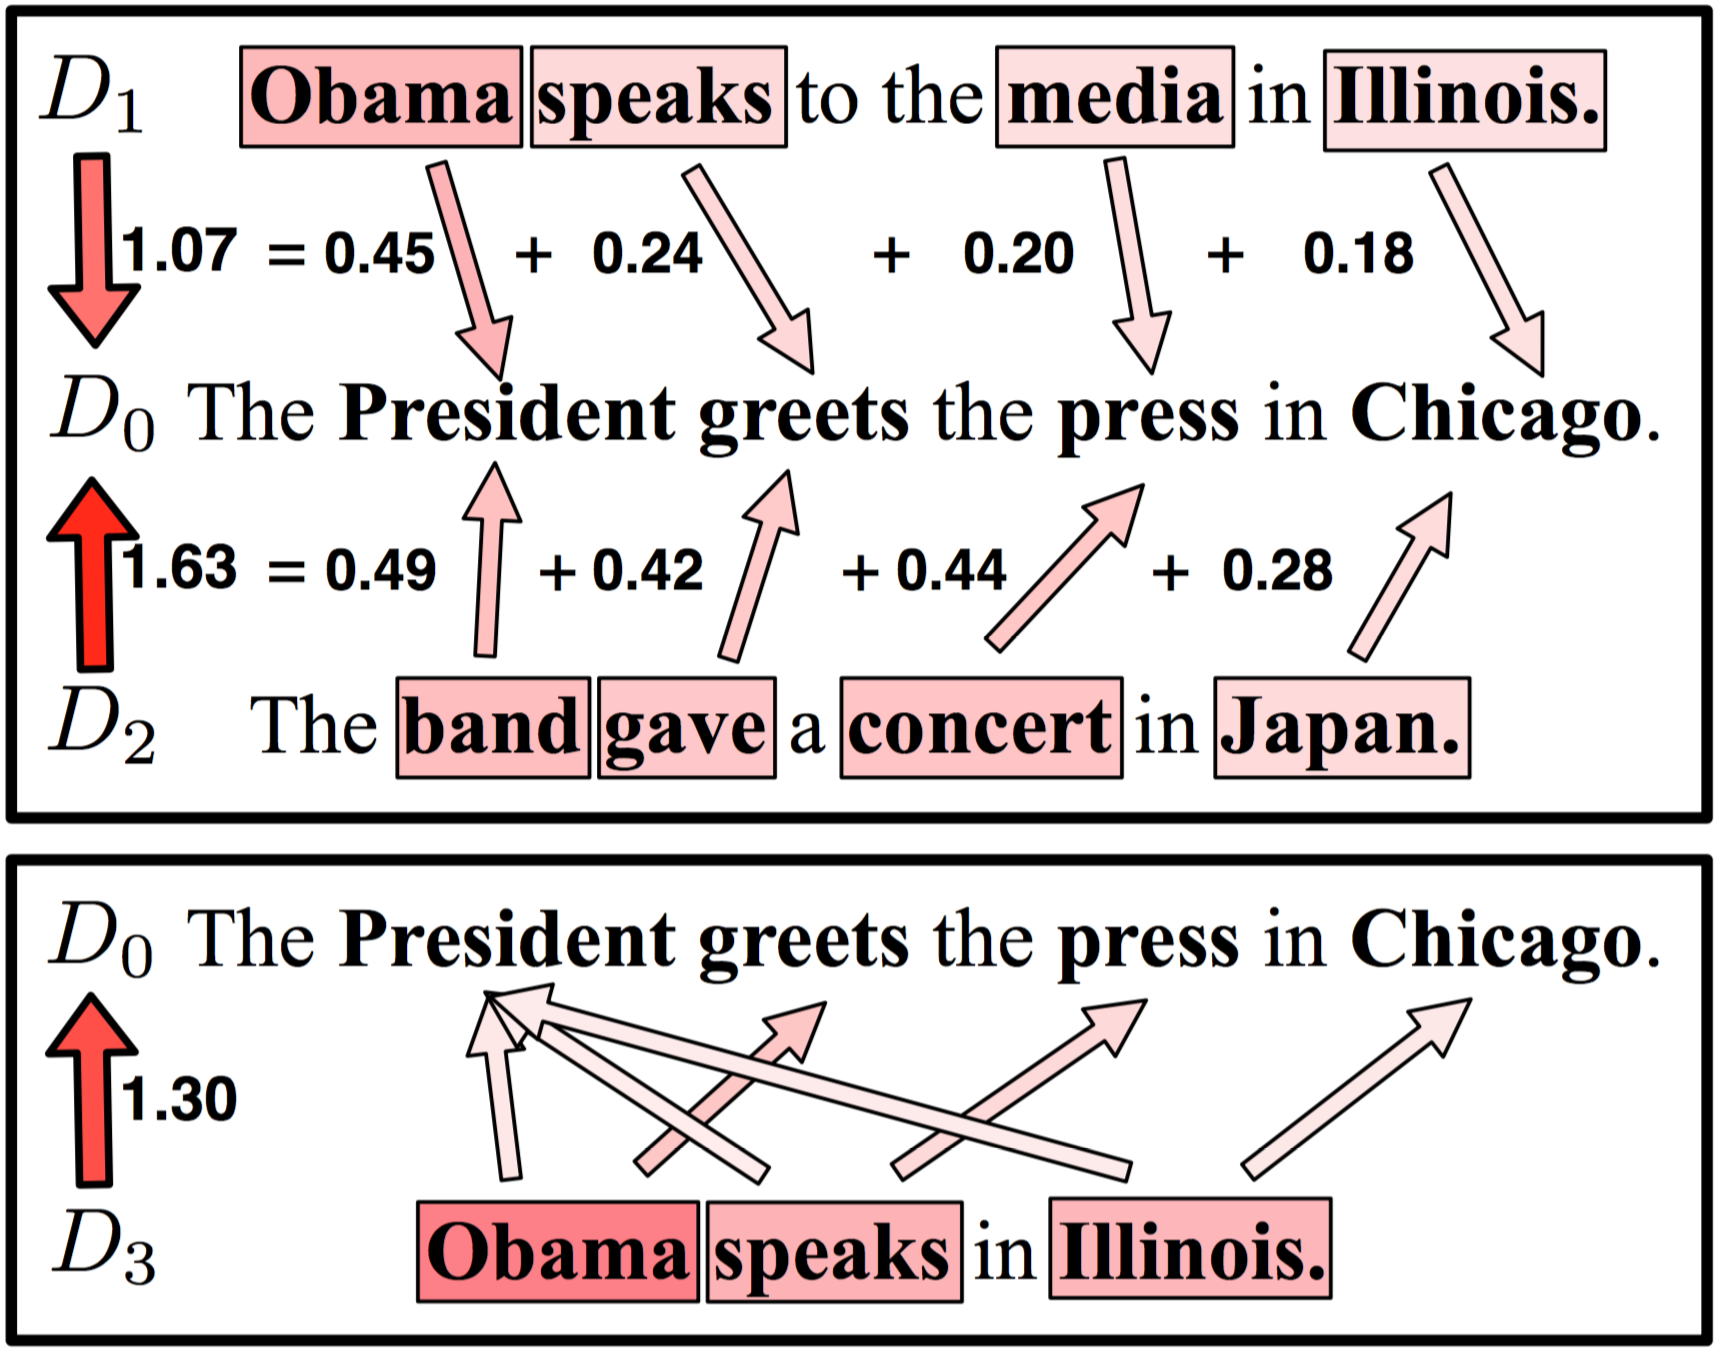
\includegraphics[width=0.4 \textwidth]{1.png}
\end{center}
\end{frame}

%------------------------------------------------
\begin{frame}
\frametitle{Оптимизационная задача}

Таким образом мы можем определить расстояние между текстами как минимальную совокупную стоимость перехода требуемую для того чтобы перевести $d$ в $d'$.

Формально данная задача минимизации стоимости перехода из $d$ в $d'$ записывается следующим образом:

$$
\min_{T \geq 0} \sum_{i,j} T_{ij} \| x_i - x_j\|_2
$$

$$
\sum_{j = 1}^n T_{ij} = d_i\  \forall i \in {1, ..., n}
$$

$$
\sum_{i = 1}^n T_{ij} = d_j\  \forall j \in {1, ..., n}
$$


\end{frame}

%------------------------------------------------



\begin{frame}
\frametitle{Word Mover's Distance}
Свойства метрики:
\begin{itemize}
\item Не имеет гиперпараметров, проста для понимания и использования
\item Демонстрирует высокие показатели метрики accuracy на реальных задачах классификации текстов
\end{itemize}
\end{frame}

\begin{frame}
\frametitle{Пример работы метрики}
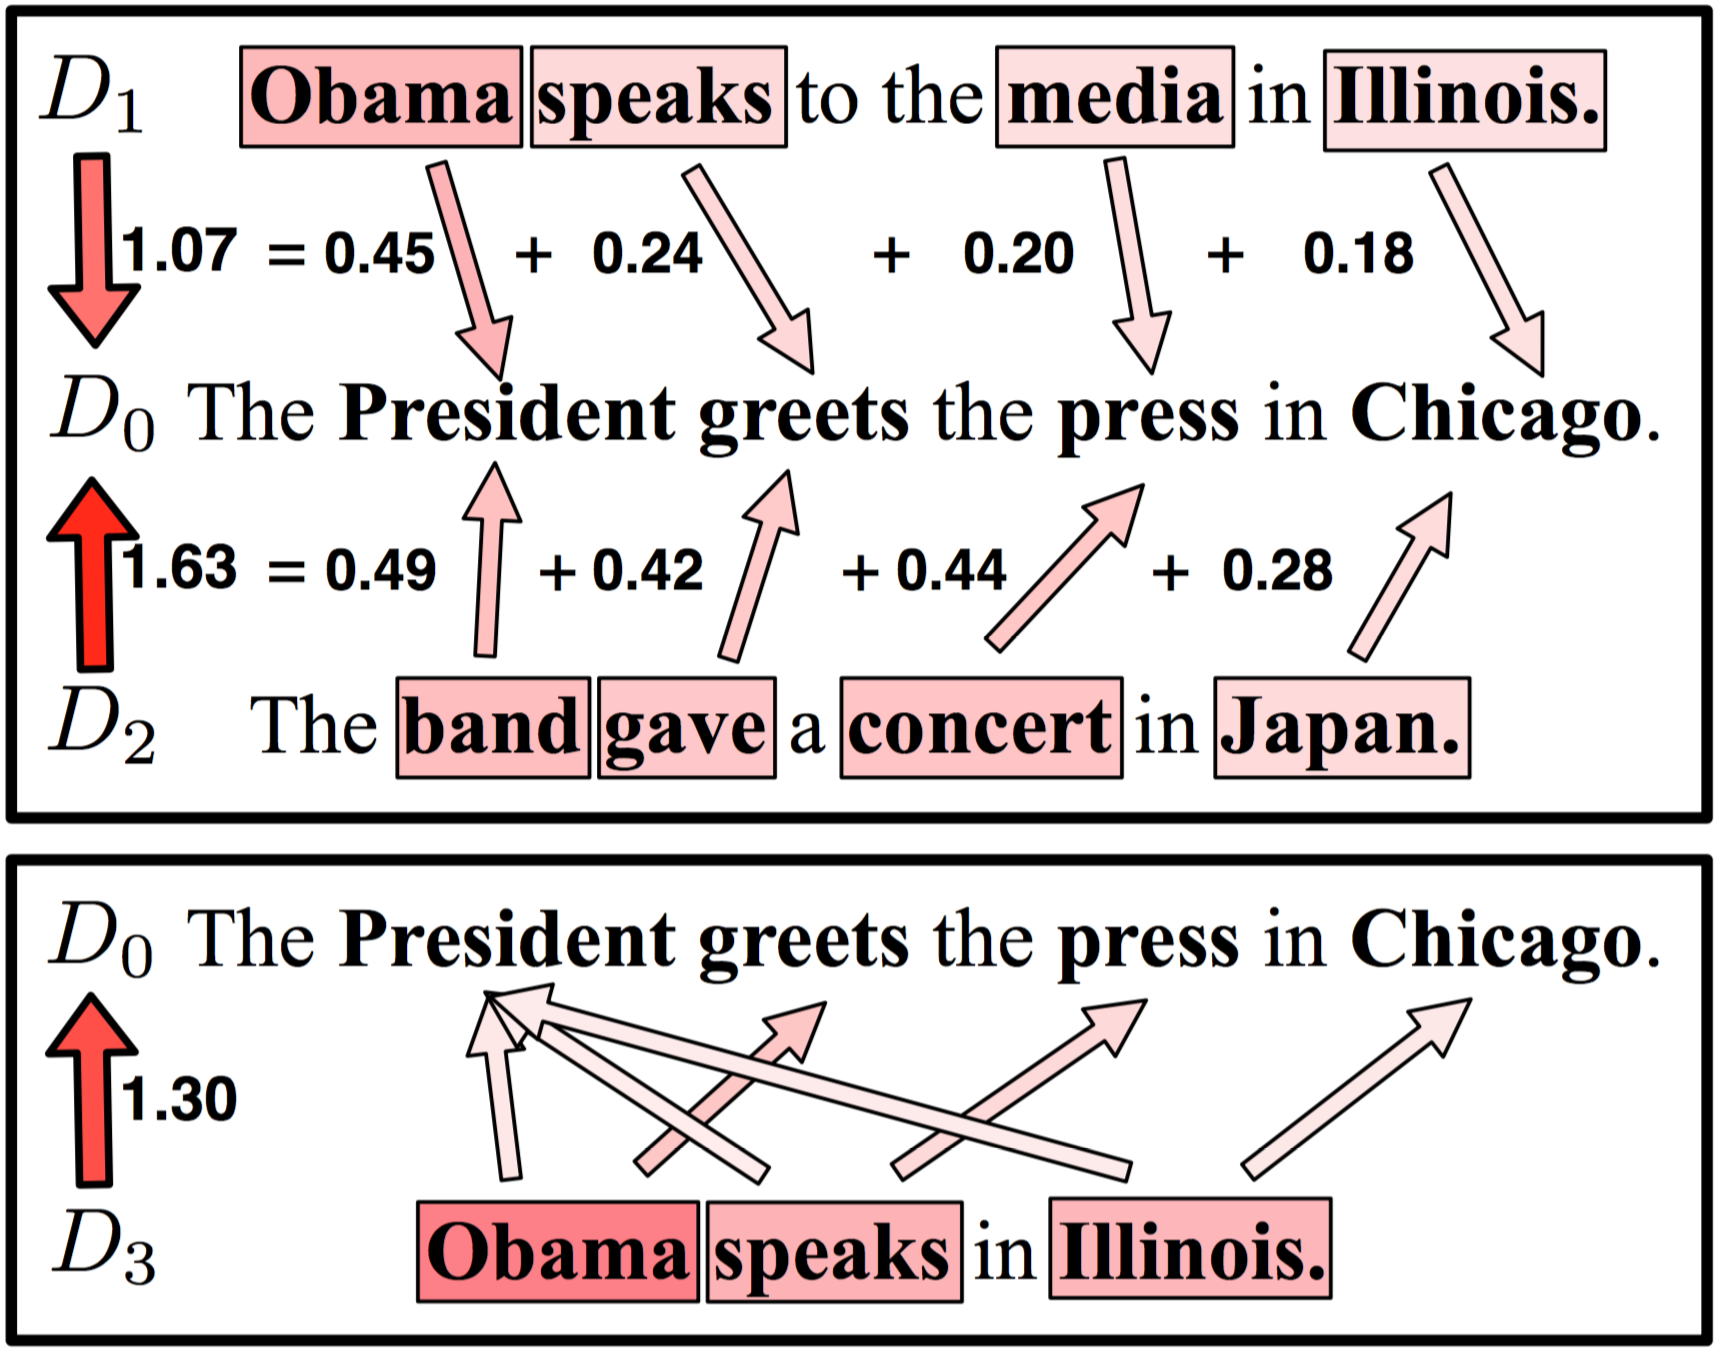
\includegraphics[width=0.7 \textwidth]{1.png}

\end{frame}

%------------------------------------------------
\begin{frame}
\frametitle{Сложность}

Решение данной задачи оптимизации имеет сложность $O(p^3log p)$, где $p$ -- количество различных слов в тексте. В больших датасетах количество уникальных слов велико -- что делает вычисление метрики долгим.

Поэтому надо как то оценивать WMD, что бы уменьшить сложность алгоритма.


\end{frame}

%------------------------------------------------
\begin{frame}
\frametitle{Word centroid distance}

Попробуем оценить значение метрики снизу:


$$
\sum_{i,j=1}^n T_{ij} c(i,j) = \sum_{i,j=1}^n T_{ij} \|x_i - x'_j \|_2 = \sum_{i,j=1}^n \|T_{ij} (x_i - x'_j) \|_2 \geq
$$

$$
\geq \| \sum_{i,j=1}^n T_{ij} (x_i - x'_j) \|_2 = \| \sum_{i=1}^n \left(\sum_{j=1}^n T_{ij}\right) x_i - \sum_{j=1}^n \left(\sum_{i=1}^n T_{ij}\right) x
'_j \|_2 =
$$

$$
= \| \sum_{i=1}^n d_i  x_i - \sum_{j=1}^n d_j x'_j \|_2 = \| Xd - Xd'\|_2
$$

Сложность вычисления данной метрики $O(dp)$, где $d$ -- размерность пространства word2vec.

\end{frame}

%------------------------------------------------
\begin{frame}
\frametitle{Relaxed word moving distance}
Несмотря на то, что WCD можно посчитать эффективно по времени, она не очень хорошо оценивает нашу метрику.

Ослабим условия задачи
$$
\min_{T \geq 0} \sum_{i,j} T_{ij} c(i,j)
$$
$$
\sum_{j = 1}^n T_{ij} = d_i\ \forall i \in {1, ..., n}
$$

Решение полученной задачи оптимизации:

$$
T^*_{ij} =
\begin{cases}
       d_i\ if\ j = \text{argmin}_j c(i,j) \\
       0,\ otherwise
\end{cases}
$$

$$
\sum_{j} T_{ij} c(i,j) \geq \sum_{j} T_{ij} c(i,j^*)  =   c(i,j^*) \sum_{j} T_{ij} = c(i,j^*) d_i = \sum_{j} T^*_{ij} c(i,j)
$$

\end{frame}

%------------------------------------------------
\begin{frame}
\frametitle{Классификация документов}

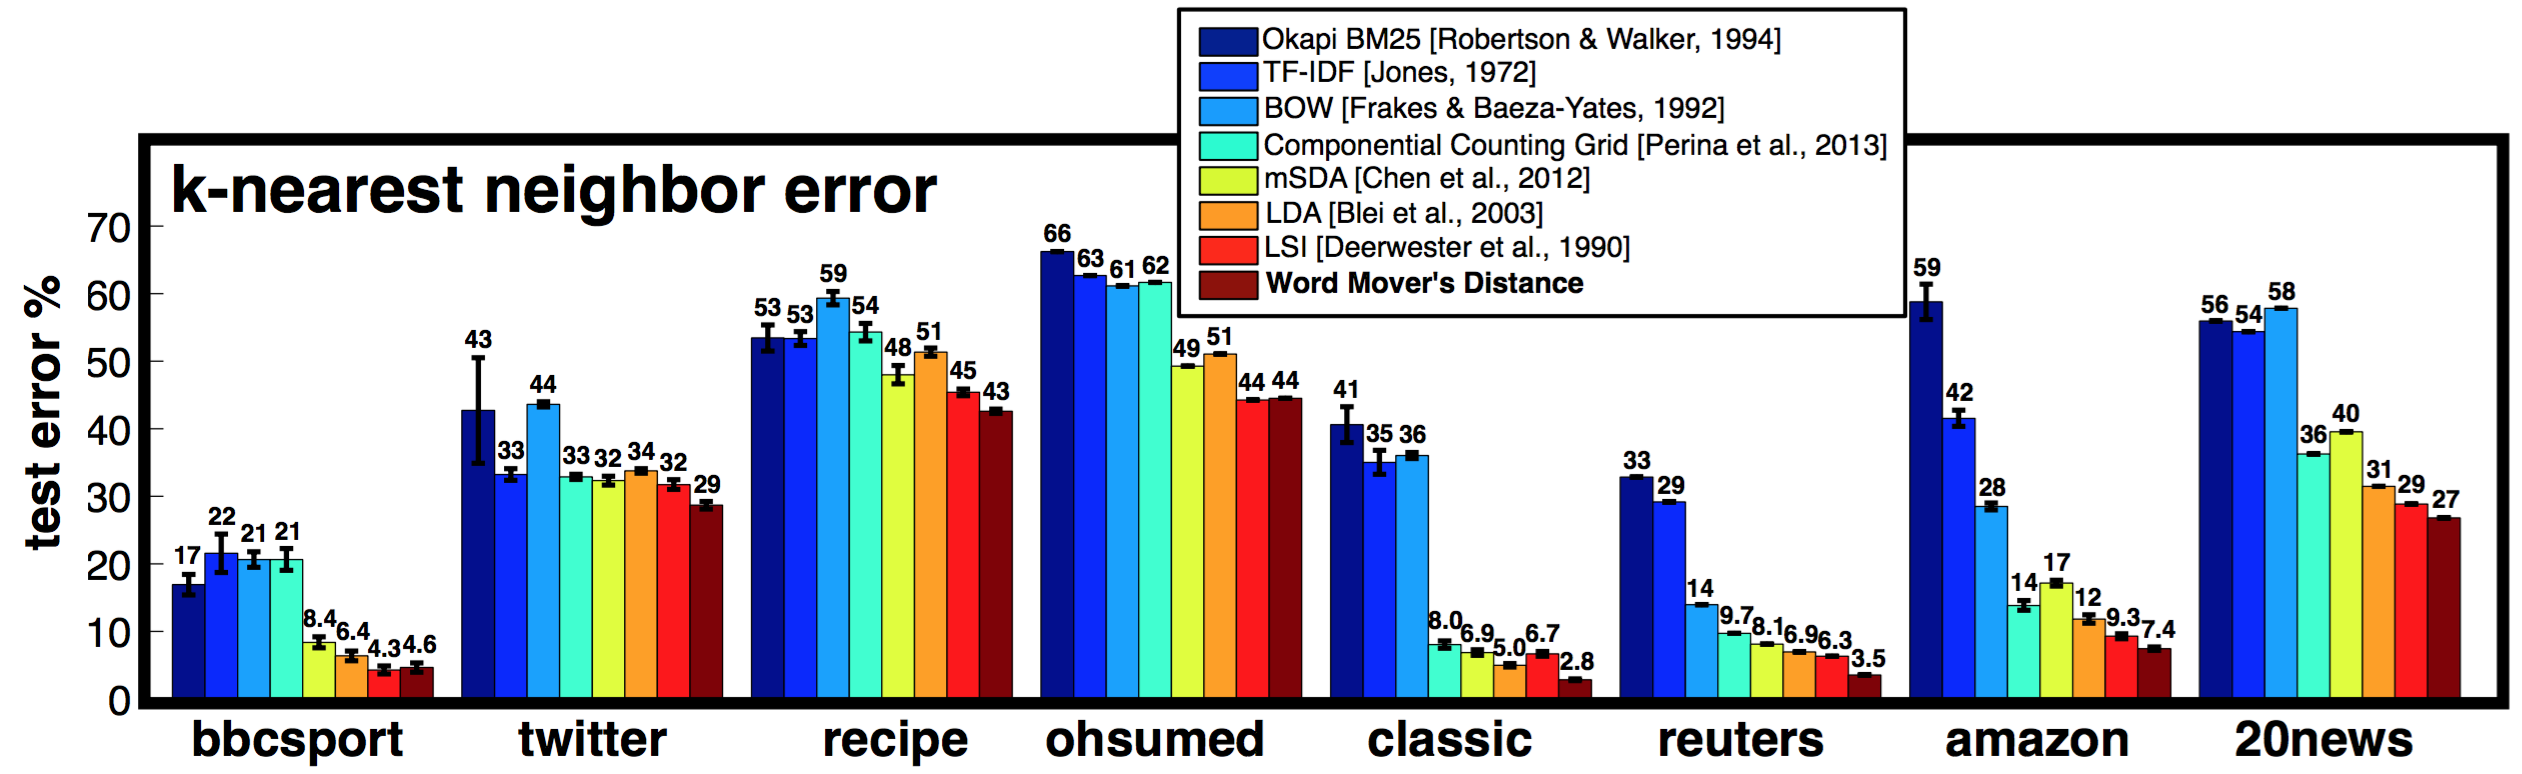
\includegraphics[width=1 \textwidth]{3.png}

\end{frame}


%------------------------------------------------
\begin{frame}
\frametitle{Классификация документов}

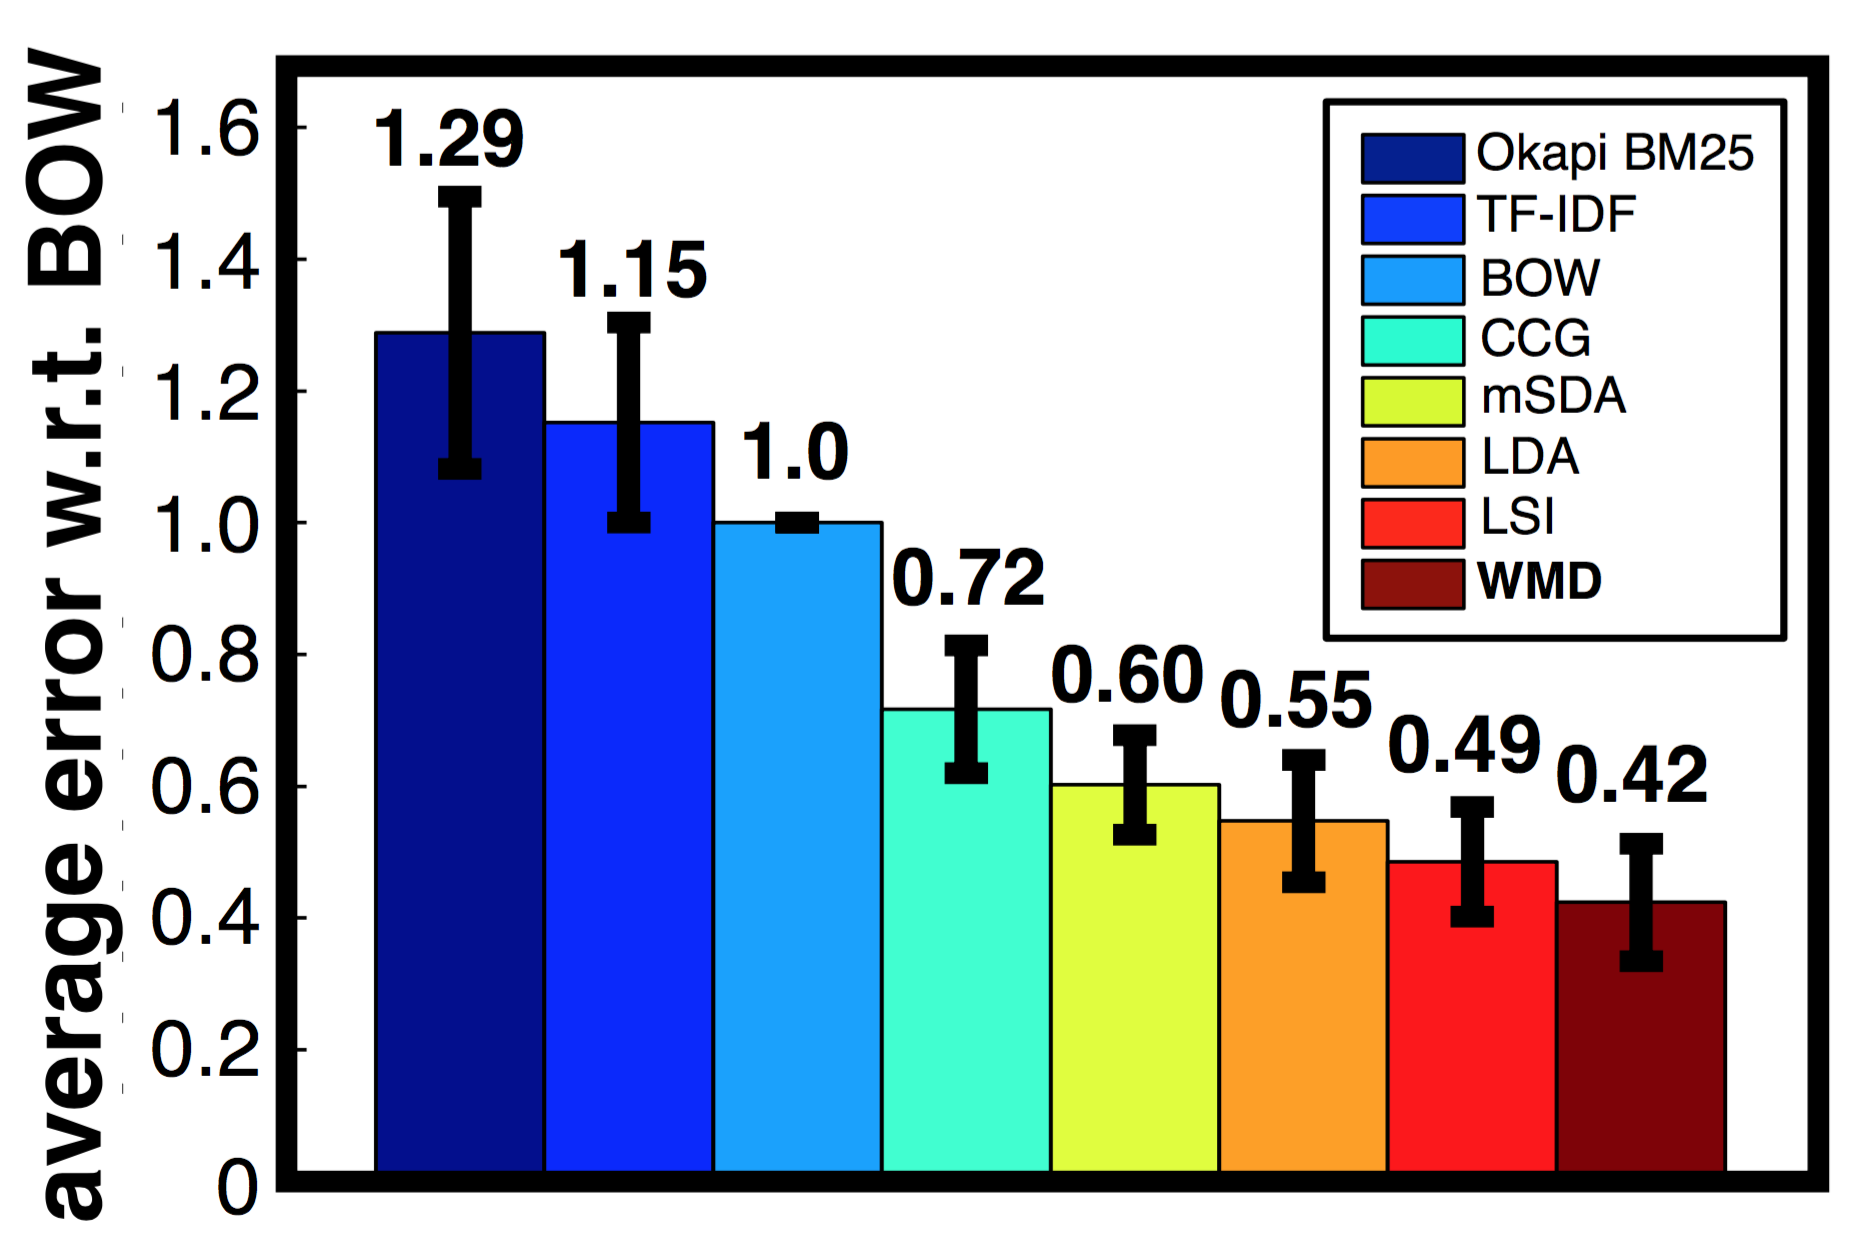
\includegraphics[width=1 \textwidth]{4.png}

\end{frame}


%------------------------------------------------
\begin{frame}
\frametitle{Оптимизация kNN}

Алгоритм:

1. Сортим все документы по возрастанию метрики WCD

2. Вычисляем WMD для первых k документа из предыдущего шага

3. Проходимся по каждому документу с k по k + m и если RWMD данного документа меньше WMD k-ого, то добавляем его в k ближних, считает для него WMD, сортим все k + 1 и отбираем из них лучший.

4. Повторяем шаг 3 пока не перестанем находить документ лучший k-ого

ч\end{frame}

%------------------------------------------------
\begin{frame}
\frametitle{Оптимизация kNN}

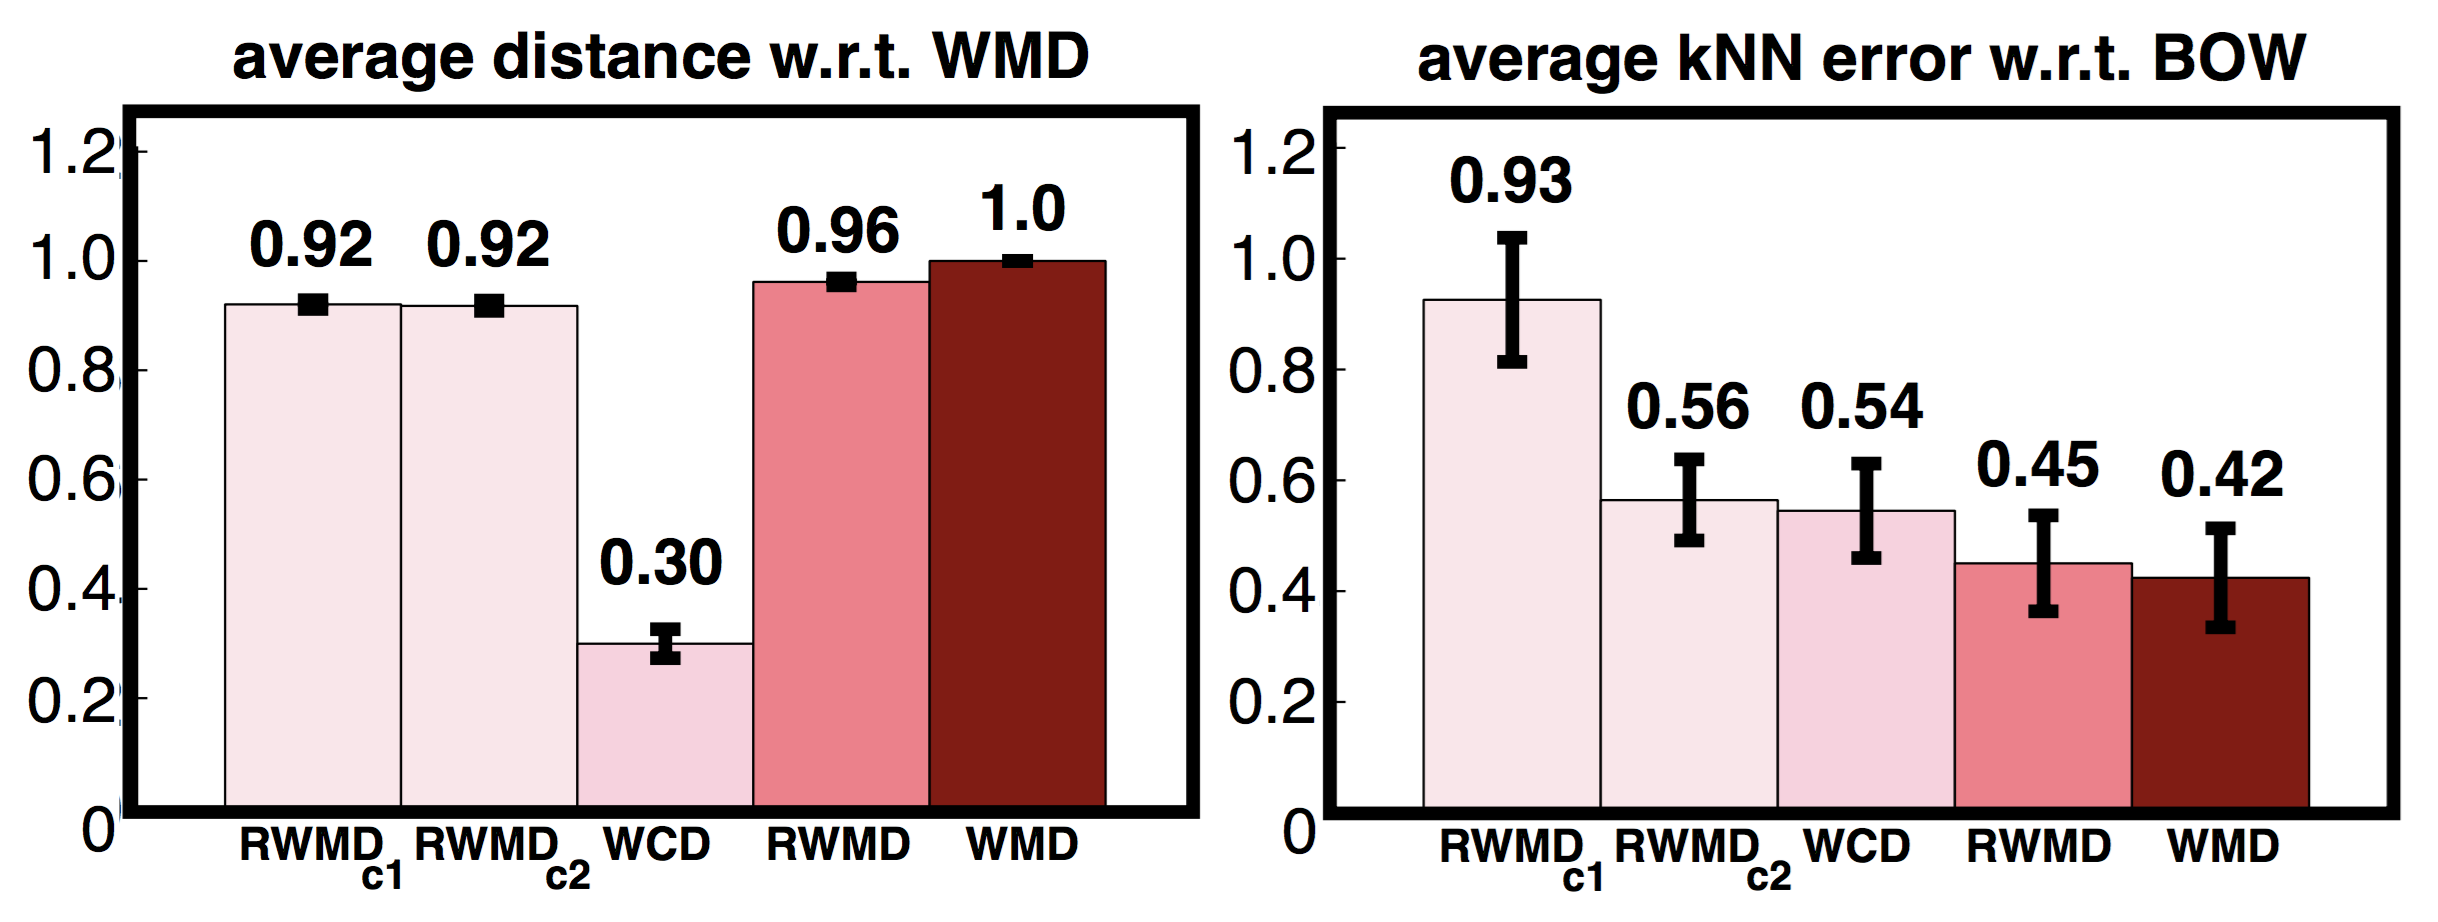
\includegraphics[width=1 \textwidth]{6.png}
\end{frame}

%------------------------------------------------
\begin{frame}
\frametitle{Оптимизация kNN}

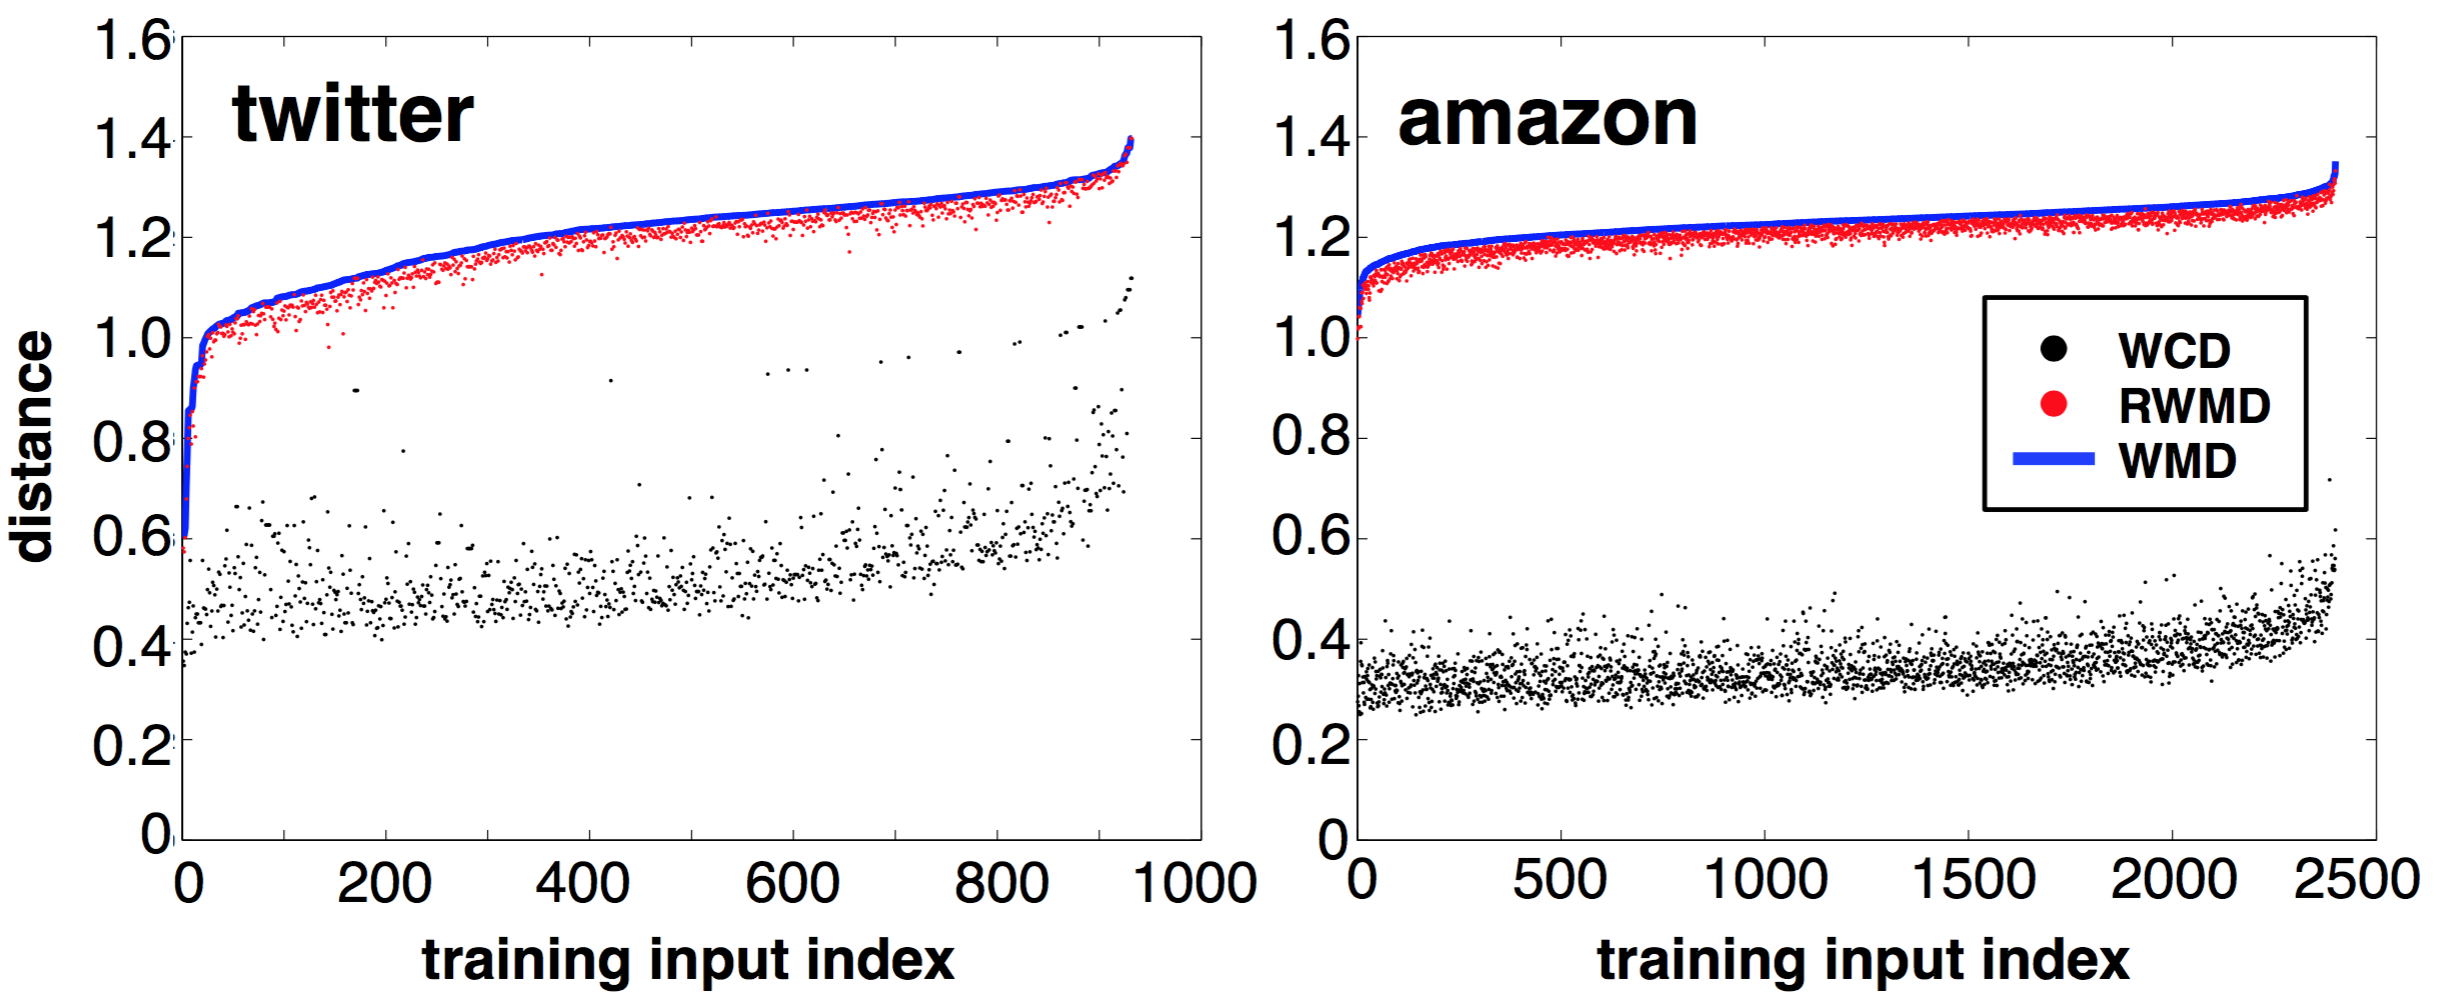
\includegraphics[width=1 \textwidth]{7.png}

\end{frame}

%------------------------------------------------
\begin{frame}
\frametitle{Оптимизация kNN}

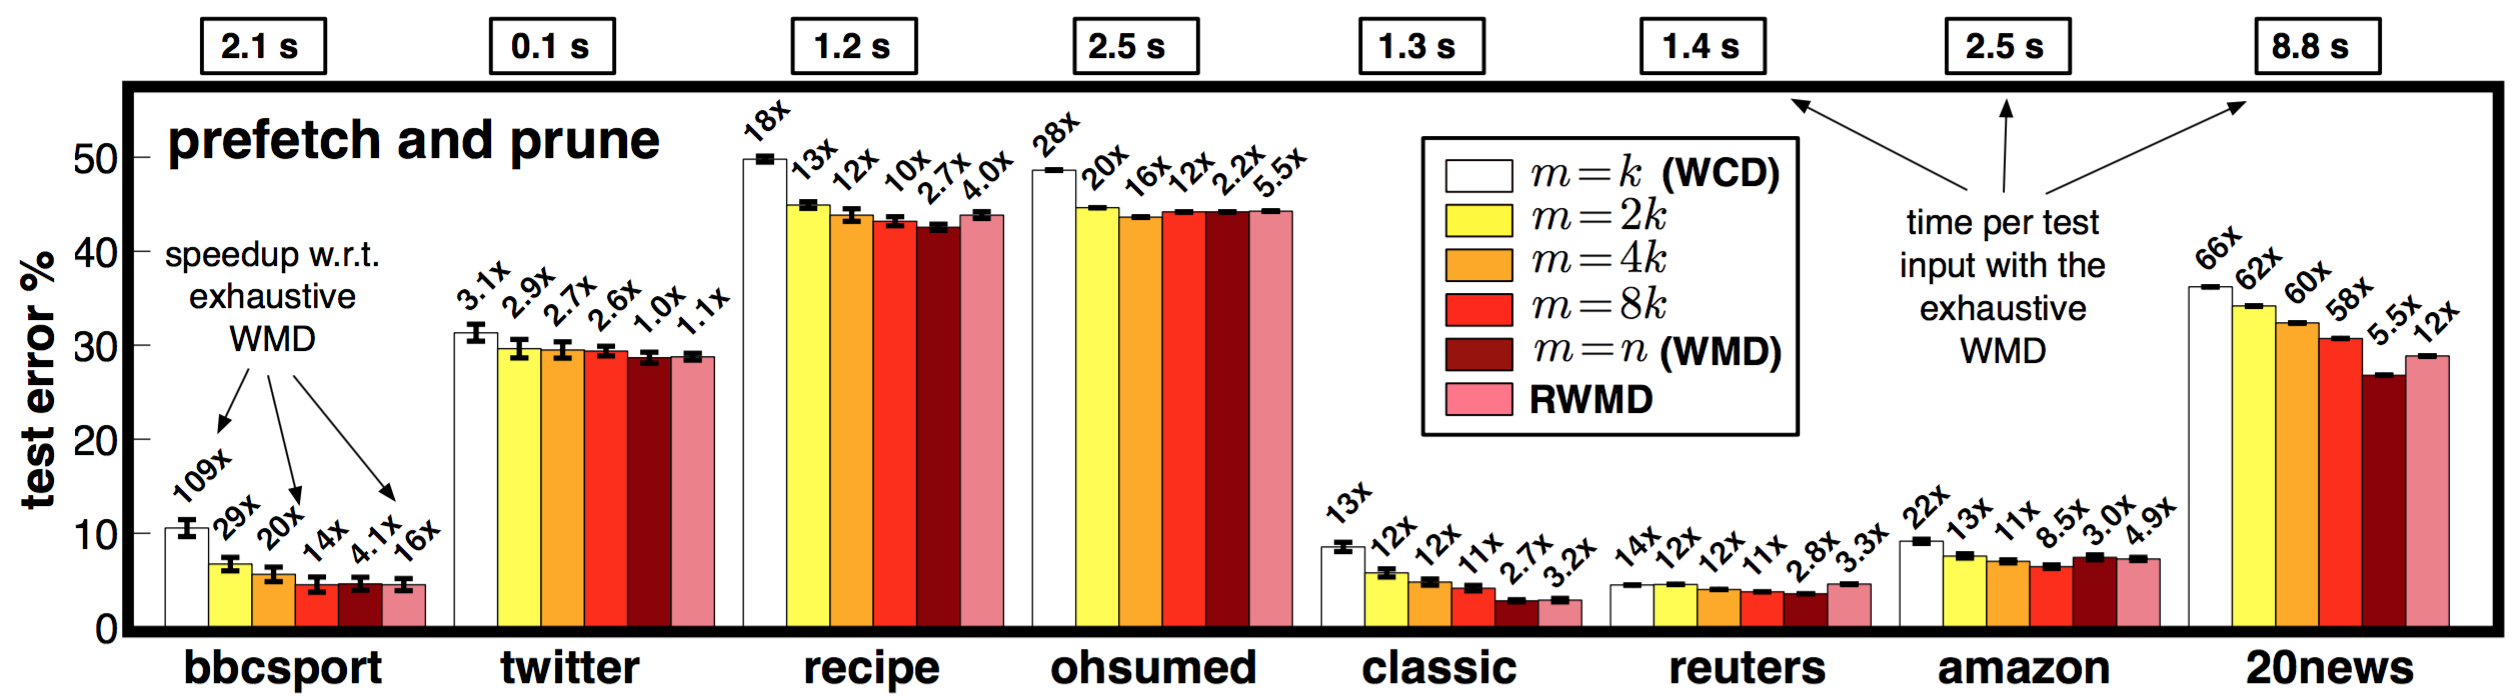
\includegraphics[width=1 \textwidth]{8.png}

\end{frame}


%------------------------------------------------
\section{Supervised Word Mover's Distance}
%------------------------------------------------





%------------------------------------------------

\begin{frame}
\Huge{\centerline{Спасибо за внимание =)}}
\end{frame}

%----------------------------------------------------------------------------------------

\end{document}
